%%%%%%%%%%%%%%%%%%%%Tesis File%%%%%%%%%%%%%%%%%%%%%%%%%%%%%%%%%%%%%%%%%%%%%%%%%%%%%

\documentclass[12pt]{book}
\usepackage{cite}
\usepackage{amssymb}
\usepackage{amsthm}
\usepackage{amsmath}
\usepackage[pdftex]{graphicx}
\usepackage{setspace}
\usepackage{mathrsfs}
\usepackage{float}

%Theorems
\newtheorem{definition}{Definition}




%Commands
\newcommand{\E}{\mathbb{E}} %Expectation
\newcommand{\tvs}{\mathscr{X}} %TVS symbol







\begin{document}
\setlength{\unitlength}{1 cm} %Especificar unidad de trabajo
\thispagestyle{empty}
\begin{center}
    %\begin{picture}(18,4)
    %\centering
    \includegraphics[scale=0.5]{log.png} \\[1cm]
    %\end{picture}
\textbf{{\LARGE Simon Fraser University}\\[0.5cm]
{\LARGE Faculty of Sciences, Math Department}}\\[1.25cm]
\begin{doublespace}
{\huge \textbf{Here comes the title}}\\[1.5cm]
\end{doublespace}
{\large Juan Gabriel Garc{\'i}a Osorio}\\[1cm]
Advisor: John Stockie\\[1cm]
Co-advisor: Paul Tupper\\[1cm]
Burnaby B.C - May  2017
\end{center}

\newpage
\tableofcontents


%%%%%%%%%%%%%%%%%%%%%%%%%%%%%%%%Chapter 0 %%%%%%%%%%%%%%%%%%%%%%%%%%%%%%%%%%%%%%%%%%%%%%%%%%%%%%%
\chapter*{Acknowlegments}

\newpage


%%%%%%%%%%%%%%%%%%%%%%%%%%%%%%%Chapter 1: Introduction %%%%%%%%%%%%%%%%%%%%%%%%%%%%%%%%%%%%%%%%%%
\chapter{Introduction}

\newpage

%%%%%%%%%%%%%%%%%%%%%%%%%%%%%%Chapter 2: Theoretical and Computational Framework %%%%%%%%%%%%%%%%
\chapter{Theoretical and Computational Framework}
%\pdfmarkupcomment[markup=Squiggly,color=green]{what eve}{Change this shit}


The foundations of the strategy we are going to use  to estimate parameters and solve inverse problems
  lies in the 
framework of Bayesian statistics. Unlike orthodox statistics, in the Bayesian approach, randomness
is a measure of uncertainty, is not a matter of frequency \cite{jaynes2003probability}. 


%Talking about Bayes rule
In real life uncertainty with respect to a measurement or a quantity of interest is usually 
connected  with the uncertainty associated to other variables and the nature of  the 
problem under study. Bayesian theory provides a solid framework to underpin the relation between
different quantities and its associated uncertainty, using whatever information
is available. The bridge that connects the previous idea
with the mathematical language is the so-called Bayes formula 
\begin{equation}\label{eqnBayes}
P(A|B)=\frac{P(B|A)P(A)}{P(B)}.
\end{equation}
Mathematically  $A$ and $B$   are subsets of some sample space $\Omega$.
$P$ is a probability measure defined on some $\sigma$-algebra of  $\Omega$.
To introduce  some language, the term $P(B|A)$ is called the likelihood, $P(A)$ is called the prior and
$P(B)$ is just a constant that normalizes to one the integral
\begin{equation*}
\int_{\Omega} P(A|B)dP.
\end{equation*}
The term $P(A|B)$ is called the posterior.

 In plain
english what formula (\ref{eqnBayes}) says is: \textbf{to know the uncertainty associated with the variable $A$
given that you know what happened with varaible $B$ it is necessary to know what would be the uncertainty
associated with the variable $B$ assuming that you know what happened with variable $A$ and that
weighted by how much uncertainty do you have about the variable $A$}.
\newline



%Ilustratory example
This interpretation of Bayes formula serves as a motivation to use it in the field of inverse problems. 
To illustrate this idea consider the following example: it's a beautiful morning, you are just chilling 
out at your place and them BAM! a rock smash the front window of your house. You want to know who threw
the rock, so your first question to solve is. Where was the rock thrown? In this scenario you can
think of $A$ and $B$  in formula (\ref{eqnBayes}) as
\begin{center}
$A$=x,y,z coordinates where the rock was thrown.\newline
$B$=x,y,z coordinates where the rock hit the window.
\end{center}
In this case Bayes formula is telling us that if we want to know where the rock was thrown given that we 
know the coordinates where the rock hit the windows (finding the posterior $P(A|B)$), we need to assume that we know
where was actually the rock thrown and estimate how likely is that, from that assumed position the rock 
would hit in the place where it did (finding the likelihood $P(B|A)$). For different suppositions of where the rock
was thrown. We need to weight that with how much do we  believe about the real position where the rock
 was actually thrown 
(choosing the prior $P(A)$).
\newline



Let's evaluate how we could tackle each one of the problems mentioned above. First to find the likelihood
we need to know how the hit position of the rock  in the window  is related to the location where it was
thrown. If we treat air resistance as a source of uncertainty in our calculations we can use
the kinematics equations of physics for parabolic trajectories, i.e.
\begin{equation}\label{eqnKinematics}
\vec{r}=\vec{r_{0}}+\vec{v_{0}}t+\frac{1}{2}\vec{g}t^{2},
\end{equation} 
where $\vec{r},\vec{r_{0}}$ are the final and initial position of the rock respectively, $\vec{v_{0}}$ is 
the initial velocity the rock was thrown and $\vec{g}$ is the gravity vector. The scalar $t$ represents time.
Now in a more physical language, to estimate the likelihood is equivalent to estimate $\vec{r}$ (where the 
rock hit the window) assuming we know $\vec{r}_{0}$ (where it was thrown). However the problem now complicates, since
we also need to estimate the initial velocity of the rock $\vec{v_{0}}$. Estimating $t$ is not a problem
since once all the other variables are estimated the value of $t$ is known. 

We are aware of the fact
that equations in physics are just models of reality and as such is just an approximation to it. To take
that into account we add an extra layer to the model by adding some noise, we propose 
\begin{equation*}
\vec{r}=\vec{r_{0}}+\vec{v_{0}}t+\frac{1}{2}\vec{g}t^{2}+\vec{\epsilon},
\end{equation*} 
where $\vec{\epsilon}$ is a random vector distributed as $\vec{\epsilon}\sim\mathscr{N}(0,\sigma I)$. Here $I$
represents the $3\times 3$ identity matrix and $\sigma>0$ is related to how much we believe in the accuracy
of equation (\ref{eqnKinematics}).  By introducing a random variable into the model
we can now think that all the variables involved 
are random variables too, that is, we now look at the  associated stochastic equation,
 therefore we can change the notation in equation (\ref{eqnBayes}) to 
the more suggestive (assuming no prior relation between $\vec{r}_{0}$ and $\vec{v}_{0}$)
\begin{equation*}
P(\vec{r_{0}}|\vec{r},\vec{v_{0}})=\frac{P(\vec{r}|\vec{r_{0}},v_{0})P(\vec{r_{0}})}{P(\vec{r}|\vec{v}_{0})}.
\end{equation*}



The nice aspect about the way we introduce the  uncertainty term  is that it can be shown that 
the following holds \cite{Somersalo}
\begin{equation*}
\vec{r}|\vec{r_{0}},\vec{v}_{0}\sim \mathscr{N}(\vec{r}_{0}+v_{0}t+\frac{1}{2}\vec{g}t^{2},\sigma I).
\end{equation*}

This means that assuming a Gaussian noise we automatically get the distribution  for the likelihood. 
We now turn our attention to model the prior.

Going back to  our hypothetical
scenario where we are chilling at our place and a rock smashed our window. We recall
that  have a very annoying neighbor in 
front of our house. He is known for being a very aggressive person, so he is our main suspect. We have the hunch
that the rock was thrown from his bedroom or at least near to it. One way to model this hunch is assuming
\begin{equation*}
\vec{r_{0}}\sim\mathscr{N}(\vec{x},\lambda I),
\end{equation*}
where $\vec{x}$ is the coordinate vector of the center of mass of his room and $\lambda$ represent how much do we believe
the rock was thrown exactly from the point $\vec{x}$. This is one way to model the prior for our problem.

Finally for the normalization constant we choose $P(\vec{r}|\vec{v}_{0})$ to be such that
\begin{equation*}
\int_{\mathbb{R}^{3}}P(\vec{r_{0}}|\vec{r},\vec{v}_{0})d\vec{r_{0}}=1\Rightarrow 
P(\vec{r}|\vec{v}_{0})=\int_{\mathbb{R}^{3}}P(\vec{r}|\vec{r_{0}},\vec{v}_{0})P(\vec{r_{0}})d\vec{r_{0}}.
\end{equation*} 


To evaluate our model, we decide to write a computer code that simulates (\ref{eqnKinematics}) for a wide range of different values
of $\vec{r},\vec{v_{0}}$ fixing $\vec{r_{0}}$. Then simulate (\ref{eqnKinematics}) fixing a different value 
of $r_{0}$ and simulating for the same range of $\vec{r},\vec{v_{0}}$ and so on. With the data obtained from
the simulation we can finally evaluate the posterior $P(\vec{r_{0}}|\vec{r},I)$. Recalling that in general
the posterior is a probability density, we can use it to estimate in several ways, what we consider to be
the best estimate of where the rock was thrown and the  uncertainty attached to that estimate .
 For instance we can pick
any of these estimates \cite{Somersalo}
\begin{eqnarray*}
\vec{r}_{MAP}=argmax_{\vec{r_{0}}\in\mathbb{R}^{3}} P(\vec{r_{0}}|\vec{r}), \\ 
\vec{r}_{CM}=\int_{\mathbb{R}^{3}} \vec{r_{0}}P(\vec{r_{0}}|\vec{r})d\vec{r_{0}},\\
\vec{r}_{ML}=argmax_{\vec{r_{0}}\in\mathbb{R}^{3}}P(\vec{r}|\vec{r_{0}}).
\end{eqnarray*} 
In these equations $\vec{r_{MAP}}$ is known as the maximum a posteriori estimate, $\vec{r}_{CM}$ is the 
conditional mean estimate and $\vec{r}_{ML}$ is the maximum likelihood estimate.
\newline

Voil{\'a}! We solved our crime, we have a way to estimate where the rock was thrown and a way to measure how
confident we are about it. The posterior is what is called a solution in Bayesian inverse problems.
\newline


%Caveats of computing complex models
Unfortunately in real life things are not as easy as  were described here in the above example. 
In reality we have to deal with several issues such as
\begin{enumerate}
\item Uncertainties in experimental measurements difficult to assess.
\item Not enough information to create a reliable estimate.
\item Computational complexity of the physical model makes prohibitive too many simulations.
\item The dimensionality of the probabilities involved is high so sampling from them is far from trivial.
\item Evaluating any of the possible estimates for the quantity of interest might be very hard.
\end{enumerate}
Just to name a few of the issues that arises when dealing with Bayesian inverse problems. To solve each
one of this issues we have available tons of different approaches. In the problem described in the 
introduction of this work (Chapter 1), all of the issues mentioned above come into play. In this chapter we are
going to discuss from a theoretical and computational point of view how to deal with issues 
3, 4 and 5 of the list.


%%%%Dealing with computational complexity
\section{Dealing with  the computational complexity of the physical model}
Physical models of the reality are usually complex and when numerically simulated, are computationally intense.
Following O'Hagan in \cite{o2006bayesian}, we can think of a physical or mathematical model as a function
$f(\cdot)$ that takes a vector $x$ of inputs and gives back a vector $y$ of outputs. But as mentioned before 
models are just that, models, so the question is: how to evaluate the uncertainty associated to the model? 
Of course when we talk about uncertainty we are talking about every possible source of randomness in the 
model or  lack of information of it. That is, the use of the word uncertainty in this work
 is related to either
epistemic or aleatory \cite{kennedy2001bayesian}.
\newline

Besides uncertainty there is another very important concept: sensitivity. When looking at a  model's performance
it is critical to assess how changes or uncertainties 
 in the input $x$ affect the output $y$. Therefore if we assess sensitivity
of the model we can assess uncertainty of the outputs. One more reason one might be interest in performing
a sensitivity analysis is to detect what variables are relevant and what variables are not, allowing to reduce
the dimensionality of the problem .

As mentioned in the introduction chapter the physical model we are dealing with is complex 
and computationally intense.
This means that assessing the uncertainty and sensitivity  associated via classical methods as in 
\cite{saltelli2000sensitivity} is not feasible.Here is where the concept of emulator as defined in \cite{o2006bayesian} comes into play. The idea is to 
approximate the function $f(\cdot)$ with an approximation function $\hat{f}(\cdot)$. But the approximation
is not any approximation, is what we call and statistical approximation. The idea of this statistical 
approximation is to associate a probability distribution to each value $f(x)$ then take the mean
of this distribution as $\hat{f}(x)$, for example.
\newline
Now that we have an idea of what we want as an approximation for the emulator, how can we construct it?
Following \cite{o2006bayesian} the idea to create the emulator is a process that satisfies
\begin{itemize}
\item At points $x$  were we know the output of the physical model i.e. $f(x)$  we want to approximate
the emulator at those points should satisfy $\hat{f}(x)=f(x)$ with uncertainty zero.
\item For the points $x^{*}$ where we don't know the output $f(x^{*})$, the emulator should
give back an estimate $\hat{f}(x^{*})$, based on the distribution for $f(x^{*})$. 
That estimate should reflect the uncertainty associated with
the interpolation/extrapolation done at that point.
\end{itemize} 


%Talking about Gaussian processes

In Bayesian analysis of computer code output one of the methods to produce an emulator with the desired
extrapolation/interpolation properties is what is known as a  Gaussian process (GP). 

\subsection{Gaussian Processes}

\begin{definition}\label{dfnGP}
A GP is a collection of random variables $\{f(x)\}_{x\in X}$, for some index family $X$,
 such that any finite set of them has a jointly
Gaussian distribution \cite{rasmussen2006gaussian}. 
\end{definition}

A GP is specified by two quantities, the mean function and the covariance function. 
Following the same notation as in Rasmussen \cite{rasmussen2006gaussian} we set
\begin{eqnarray*}
m(x)=\E(f(x)),\\
k(x,x')=\E((f(x)-m(x))(f(x')-m(x'))).
\end{eqnarray*}
So if $\{f(x)\}$ is a GP with mean $m(x)$ and covariance $k(x,x')$ we will write
\begin{equation*}
f(x)\sim \textbf{GP}(m(x),k(x,x')).
\end{equation*} 

To understand the notion of a GP observe that what  
we are trying to do is to approximate a function $f(\cdot)$, then
the symbol $f(x)$ represents a random variable whose realizations are  the possible values of the
 function $f(\cdot)$ at $x$ and $m(x)$ is the best approximation we can do to predict the actual value 
of $f(\cdot)$ at that point $x$. The uncertainty associated to that prediction is going to be related
to the quantity $k(x,x)$.

Since we are going to use GP to fit  data in a high dimensional euclidean space, it will be convenient to think
of the set of index $X$ in definition \ref{dfnGP} as $\mathbb{R}^{n}$ for some $n\geq 1$. 
\newline

The reason why the definition of a Gaussian process is useful and powerful is because a GP is 
completely characterized by $m(x)$ and $k(x,x')$\footnote{ $k(x,x')$ 
is usually known as the kernel of the GP}\cite{lifshits2012lectures}. Therefore to fit and 
predict using GPs we only need to define just two quantities. For example the way to choose
the covariance kernel is with the aid of some real valued function. For example a very common covariance
function is given by what is called the squared exponential (SE)
\begin{equation}\label{eqnsquareexponential}
k(x,x')=e^{-\frac{1}{2}\|x-x'\|_{2}^{2}}.
\end{equation}
In this case this definition of the covariance is telling us that points that are close to each other
are highly correlated whereas far away points has a correlation that decays exponentially fast with distance.
There are some `standard' ways to choose the covariance function depending on the kind
of regularity we want for the GP fitting. To see what is the relation between regularity
of the fitting and the kernel we need to realize that once the covariance function has been 
specified we end up with a distributions over some function space. Talking 
about distribution over spaces of functions is a delicate topic that has to be done in a rigorous manner.
That is why at this point it is convenient to digress for a moment an talk about distributions in 
function spaces. The details presented here follow from \cite{lifshits2012lectures}.

\subsubsection{Distributions Over Function Spaces}
Since in general the relevant function spaces (e.g. $L^{p}$ spaces, Sobolev spaces, etc...) are 
normed vector spaces, they have a topology inherited from the metric induced by the norm, therefore 
in general, function spaces are topological vector spaces (TVS). 

If $\mathscr{X}$ is a TVS and $\mathscr{X}^{*}$ is its dual, we will denote the action of an 
element $f\in\tvs^{*}$ over an element $x\in\tvs$ as $\langle f,x\rangle$. On the other
hand we  define a random vector taking values in $\tvs$ as a measurable map 
\begin{equation*}
X:(\Omega,\mathscr{F},P)\longrightarrow\tvs,
\end{equation*}
where $(\Omega,\mathscr{F},P)$ is a probability space. To say that 
a random variable  $X$ takes vales in $\tvs$ we will write $X\in\tvs$. 
Therefore by letting $\tvs=L^{2}(\mathbb{R})$, for 
example, we now understand what does it mean $X\in L^{2}(\mathbb{R})$.

On the other hand we say that a random vector $X\in\tvs$ is called Gaussian if $\langle f,x\rangle$ is
a normally distributed random variable for all $f\in\tvs^{*}$. Observe that $x$ represents  a realization
of $X$, so the definition of a Gaussian vector in $\tvs$ makes sense. For normally
distributed random vectors in $\mathbb{R}^{n}$ we have quantities like expectation and covariance matrix.
In a more   general ( possible infinite dimensional) framework we say that a vector $a\in\tvs$ is the 
expectation of $X\in\tvs$ if 
\begin{equation*}
\E(f,X)=\langle f, a\rangle,\qquad\text{for all }f\in\tvs^{*}.
\end{equation*}
Also a linear operator $K:\tvs^{*}\longrightarrow \tvs$ is called the covariance operator (e.g covariance
matrix in the finite dimensional case) if
\begin{equation*}
cov(\langle f_{1},X\rangle,\langle f_{2},X\rangle)=\langle f_{1},Kf_{2}\rangle,
\end{equation*}
for all $f_{1},f_{2}\in\tvs^{*}$. It can be shown that the covariance operator has the same nice properties
as in the finite dimensional case, such as symmetry and non-negative definiteness. 
\newline

With the construction of a rigorous framework that allows us to talk about Gaussian distributions in 
function spaces we can see why once the covariance function and the mean function are defined then we 
have created a Gaussian distribution over some function of spaces and why the nature of the function
space depends heavily on the regularity properties of the covariance kernel. In 
this work we are going to be mainly concerned to work with kernels that are at least continuous
(For example the SE kernel in equation (\ref{eqnsquareexponential}) is $C^{\infty}$). To see why 
by just giving a recipe for the covariance and the mean defines a distribution over some function
spaces, consider the following case, which is our case of interest in this work. Since we are 
interest in at least continuous covariance functions consider $\tvs=\mathbb{C}(T)$ where 
$T\subset\mathbb{R}^{n}$ and $T$ is compact. The space of real valued continuous functions in $T$ is a Banach
space with the norm \cite{bressan1900lecture}
\begin{equation*}
\|g\|=\max_{x\in T}|g(x)|.
\end{equation*}
The dual space of $\tvs$ is given by $\tvs^{*}=\mathbb{M}(T)$ the set of sign measures on $T$. In this 
case the duality is given by 
\begin{equation*}
\langle\mu,g \rangle=\int_{T}gd\mu.
\end{equation*}
Therefore by having a GP,  $\{f(x)\}_{x\in T}$ (see definition \ref{dfnGP}) with mean function $m(x)$ and 
covariance function $k(x,x')$,  we can see the GP  as a Gaussian random variable $f\in\tvs$ with mean
and covariance operator defined as
\cite{lifshits2012lectures} 
\begin{eqnarray*}
\E(f)=m\in\mathbb{C}(T), \\
(K\nu)(s)=\int_{\mathbb{R}^{n}}k(x,x')\nu(dx'),\qquad\text{for }\nu\in\mathbb{M}(T).
\end{eqnarray*}

With this  mathematical framework to work with GP, it is possible to explain how
they work. Imagine that we have some experimental measurements or emulator results (train inputs) 
$\{(x_{i},f(x_{i}))\}_{i=1}^{m}\in\mathbb{R}^{n+1}$,
for a real valued function $f:\mathbb{R}^{n}\longrightarrow\mathbb{R}$. Having these values 
we would like to make inference on the possible values of $f$ on some set of points $\{x_{j}^{*}\}_{j=1}^{k}$ (test inputs).
Since we assumed  that $\{f(x)\}$ is a GP, that means that the vectors
\begin{eqnarray*}
\textbf{f}=\begin{bmatrix}f(x_{1}) & \ldots & f(x_{m}) \end{bmatrix}^{T}, \\
\textbf{f}_{*}=\begin{bmatrix}f(x_{1}^{*}) & \ldots & f(x_{l}^{*}) \end{bmatrix}^{T}.
\end{eqnarray*}
Have a  jointly Gaussian distribution given by  (assuming no trend in the data, i.e. mean zero).
\begin{equation}\label{eqnconditional}
\begin{bmatrix}
\textbf{f} \\
\textbf{f}_{*}
\end{bmatrix}\sim\mathscr{N}\left(0,\begin{bmatrix} K(X,X) & K(X,X_{*}) \\
						    K(X_{*},X) & K(X_{*},X_{*}) \end{bmatrix}
\right),
\end{equation}	
where $(K(X,X))_{ij}=cov(f(x_{i}),f(x_{j})), K(X,X_{*})_{ij}=cov(f(x_{i}),f(x_{j}^{*}))$ and so forth.


Since we know the vector $\textbf{f}$ and we want to make inferences about the vector $\textbf{f}_{*}$,
then we are looking for the distribution of $\textbf{f}_{*}|\textbf{f}$. By well known properties
of the multivariate Gaussian distribution we can check that \cite{lifshits2013gaussian}
\begin{equation}\label{eqnformulameancovariance}
\textbf{f}_{*}|\textbf{f}\sim\mathscr{N}\left(K(X_{*},X)K(X,X)^{-1}\textbf{f},
K(X_{*},X_{*})-K(X_{*},X)K(X,X)^{-1}K(X,X_{*})\right).
\end{equation}
So to interpolate the function along the test inputs we can choose the mean  of the distribution
of $\textbf{f}_{*}|\textbf{f}$ as the interpolant. Also we can have a good idea of how reliable if the fitting
by looking at the covariance matrix. As we can see choosing the covariance kernel to create
the covariance matrix is a crucial step in the fitting process. How do we choose the kernel?
There are some standard ways to do that and some standard kernels to choose from.
Some of the most common kernels are (setting $r=\|x-x'\|_{2}$)

\begin{itemize}
\item Gauss: $k(r;\theta)=e^{-\frac{1}{2}(\frac{r}{\theta})^{2}}$
\item Exponential: $k(r;\theta)=e^{-\frac{r}{\theta}}$\\
\item Matern $\frac{3}{2}: k(r;\theta)=(1+\frac{\sqrt{3}r}{\theta})e^{-\frac{\sqrt{3}r}{\theta}}$.
\item Matern $\frac{5}{2}: k(r;\theta)=(1+\frac{\sqrt{5}r}{\theta}+\frac{5}{3}
(\frac{r}{\theta})^{2})e^{-\frac{\sqrt{5}r}{\theta}}$.
\item Power-Exponential: $k(r;\theta,p)=e^{-(\frac{r}{\theta})^{p}}$
\end{itemize}

As we can see covariance kernels are usually defined in terms of parameters, so depending on the model
under study we can find the parameters that best suits the model. The question now is: how
to choose the right parameters for the model? Consider the following situation: we have a 
set of training points $\{(x_{i},f(x_{i}))\}_{i=1}^{n}$ and we want to predict the 
outputs $f(x)$ for some points in $x$ that is not in the training set. To do the prediction
using GPs we choose some kernel  $k(r;\theta)$ that depends on the parameter $\theta$ 
($\theta$ could be an scalar, vector, etc.). In this case to predict the values of 
$y=\{f(x_{1}^{*}),\ldots f(x_{m}^{*})\}$, we can use
Bayes rule and optimize the likelihood, mathematically we want to optimize
\begin{equation*}
p(y|\{(x_{i},f(x_{i}))\}_{i=1}^{n},\theta).
\end{equation*}
By definition \ref{dfnGP} we know that the conditional probability has to be distributed as
a multivariate normal distribution\footnote{Recall that the $n-dimensional$ Gaussian measure
$N(\mu,\Sigma)$ has
Lebesgue density given by $\frac{1}{\sqrt{(2\pi)^{n}|\Sigma|}}\exp{\left(-\frac{1}{2}(x-\mu)^{T}\Sigma^{-1}
(x-\mu)\right)}$}, hence by taking the $\log$ of the probability we get
\begin{equation}\label{eqnloglikelihood}
\log(p(y|\{(x_{i},f(x_{i}))\}_{i=1}^{n},\theta))=-\frac{1}{2}y^{T}K_{y}(\theta)^{-1}y-
\frac{1}{2}\log|K_{y}(\theta)|-\frac{n}{2}\log(2\pi).
\end{equation}
Here $K_{y}(\theta)$ is the covariance matrix associated to the GP conditional to  $\{(x_{i},f(x_{i}))\}$ 
(see equation (\ref{eqnconditional})). In this case we can see explicitly the dependence on 
the parameter $\theta$ for the  prediction of the Gaussian Process. Since we want to do 
the best possible prediction, it makes sense to try to optimize equation (\ref{eqnloglikelihood}) 
with respect to the parameter $\theta$. This gives a reliable criteria on how to tune up
the parameters of the chosen kernel. 
\newline




If we are dealing with a complex high-dimensional physical model
that is emulated by $\hat{f}$, we need to be very careful of what points to choose as our training points
for our GP. Usually training points come from the output of the simulation of the physical
model through the emulator $\hat{f}$, this is a problem. Ideally 
we would like to pick as many training points as possible to make the fitting better, but picking too many points
to do the interpolation might result in a very high computational demand, on the other hand if we pick up
just a few points to do the emulation and then do the fitting with those points, this might result in a really
bad fitting with the consequence of obtaining unreliable inferences when using GPs to fit the test points. This
shows that we need a systematic way to choose how to get the training points. We need to choose those points
in a way that we can fill as much space as possible with as few training points as possible without
sacrificing quality in the prediction for the test points. This can be accomplish
through  something known as  space filling designs. 
\newline


\subsection{Experimental Design and Sensitivity Analysis}

At this point it is clear that if we want to use GPs to fit the data obtained through an emulator 
$\hat{f}(x)$ we need to decide how many runs of the emulator we are going to do. If the domain of the
emulator is a subset of $\mathbb{R}^{n}$ then we need to decide what points in the domain we are going 
to choose as well. This is a very delicate issue since we need to find the right balance between
the number of possible emulations given time and computational power constraints
 and a good distribution in space of these training points to get a good
fitting in the output on   every test point we choose.
\newline
 
Given an set $T$, there are several ways to create space filling designs for it 
\cite{pronzato2012design}. In this work we are going to focus on maximin designs
\cite{johnson1990minimax}. To define this kind of design, consider a metric space $(T,d)$ (e.g.
$T\subset\mathbb{R}^{n}$, compact and $d$ the Euclidean distance) and any subset of $T$, 
$S$ with finite (fixed) cardinality, say $|S|=n$.
A maximim distance design $S^{o}$ is such that
\begin{equation*}
\max_{S}\min_{s,s'}d(s,s')=\min_{s,s'\in S^{o}}d(s,s')=d^{o}.
\end{equation*}
That is, we are looking for the set $S^{o}$ of cardinality $n$ that maximizes the minimum distance among 
its elements. As an example consider $T=[0,1]^{3}$, the unit cube in $\mathbb{R}^{3}$ and $n=8$, in 
that case the design that maximizes the minimum distance among its elements is given by choosing
the points that live in each of the 8 vertex of the cube. In this case $d^{o}=1$. The problem of finding
the optimum in a maximin design is hard, therefore in general is necessary to use computational tools
for optimization. In chapter 4 we will see how to use these computational tools to create
a proper experimental maximin design.

The connexion of maximin experimental designs with GP is the following. Consider the
GP $\{f(x)\}_{x\in T}$. If we fix $S$ and let $f_{s}$ to be the conditional distribution 
of $\{f(x)\}_{x\in T}$ given the realizations $f(s), s\in S$, if we let $K_{s}$ to be 
the correlation of the distribution $f(s), s\in S$. Then it can be shown
that the minimax design minimizes the quantity
\begin{equation*}
M(S)=-det(K_{s}).
\end{equation*}
Since the covariance matrix is positive defined (hence the correlation matrix is also positive defined)
, then $det(K_{s})>0$. By minimizing the  negative of the determinant  we are getting looking
for the maximum value of the determinant. This is achieved when the column vectors of a matrix
are close to orthogonal. In statistical terms what we are looking for is 
the least possible correlation between the difference points in the maximin design. Here
is where its importance lies.
\newline

 
If we have a good space filling design, then we have a good fit when using GPs to interpolate  the 
points we want to get information about. If we have a reliable fitting we have the chance
to reduce the dimensionality of the model and hence its complexity. Indeed, assume that
you want to fit a function  $f:T\subset \mathbb{R}^{n}\longrightarrow\mathbb{R}$ and you want to 
know if all the $n$ variables in the domain are relevant to understand  the behaviour of $f$. For 
example if $f$ behaves like the function $f(x_{1},\ldots,x_{n})=x_{1}+x_{2}+10^{-8}x_{3}$ on $T=[0,1]^{n}$, 
then clearly 
instead of working in an $n-$dimensional space and dealing with all its complexities we can
reduce the model to a simple $2-$dimensional one. The question is then. How to quantify the 
dependence (or sensitivity) of $f$ on $x_{1},\ldots,x_{n}$? There are multiple ways to perform such
sensitivity analysis \cite{saltelli2000sensitivity}. In this work we are going to focus on
the method  introduced
by Ilya Meyerovich Sobol. This method is what is called a variance-based Monte Carlo method (VBMCM).
The idea of a VBMCM is to use the variance produced by  the inputs of a function as an indicator of its importance.
The description of Sobol's method follows from \cite{saltelli2000sensitivity}.

Witout lost of generallity we may assume that we have a function 
$f: \Omega^{n}\subset\mathbb{R}^{n}\longrightarrow \mathbb{R}$ where $\Omega^{k}$ is the $n-$dimensional
unit cube\footnote{Since our goal is to study the behaviour of a function that is obtained by the output
of some physical experiment or simulation of it we may assume that the functions of interested in this 
work have a compact domain, hence by some reescaling we can always assume that the domain of the function
under study has as its domain the unit hypercube}. Sobol's idea was to decompose $f$ as 
\begin{equation*}
f(x_{1},\ldots,x_{n})=f_{0}+\sum_{k=1}^{n}f_{k}(x_{k})+\sum_{1\leq k< l\leq n}f_{kl}(x_{k},x_{l})+\ldots+
f_{1,2,\ldots,n}(x_{1},\ldots,x_{n}).
\end{equation*}
The functions in this decomposition cannot be arbitrary functions. First $f_{0}$ has to be a constant.
On the other hand the other functions must satisfy
\begin{equation*}
\int_{[0,1]}f_{i_{1},\ldots,i_{s}}dx_{i_{k}}=0\qquad\text{if } 1\leq k\leq s.
\end{equation*} 
Therefore by Fubinni's theorem we may conclude that functions with different subindices are 
 pairwise orthogonal in $\Omega^{n}$. The second consequence of this result is that
\begin{equation*}
\int_{\Omega^{n}}fdx=f_{0}+\int_{\Omega^{n}}\sum_{k=1}^{n}f_{k}(x_{k})+
\int_{\Omega^{n}}\sum_{1\leq k< l\leq n}f_{kl}(x_{k},x_{l})dx+\ldots+
\int_{\Omega^{n}}f_{1,2,\ldots,n}(x_{1},\ldots,x_{n})dx.=f_{0}.
\end{equation*}
So by obtaining $f_{0}$ we can use recursion to obtain the other functions in the decomposition. For example
if $dx_{\sim 1}$ represent integration with respect to $x_{2},x_{3},\ldots, x_{n}$, it is not 
hard to see that 
\begin{equation*}
f_{1}(x_{1})=-f_{0}+\int_{[0,1]^{n-1}}f(x)dx_{\sim 1}.
\end{equation*}
Similar formulas hold for the other functions in  the decomposition of $f$. By knowing explicitly all
the functions in the decomposition allows us to assess the relevance of each variable in the 
behaviour of $f$ by defining on them its variances. The total variance $D$ of $f$ is defined as
\begin{equation*}
D=\int_{\Omega^{n}}f^{2}(x)dx-f_{0}^{2}.
\end{equation*}
As we can see this is the same as the usual definition of the variance of a random variable $X$  in statistics: 
\begin{equation*}
Var(X)=\E(X^{2})-\E(X)^{2}.
\end{equation*}
Where in this case the expectation operator is obtained by taking the integral over the whole space $\Omega^{n}$.
Similarly we compute the partial variances as
\begin{equation*}
D_{i_{1},\ldots,i_{s}}=\int_{[0,1]^{n-1}}f^{2}_{i_{1},\ldots,i_{s}}dx_{i_{1}}\ldots dx_{i_{s}}.
\end{equation*}
With these variances we define the $s-th$ order sensitivity  as
\begin{equation*} 
S_{i_{1},\ldots,i_{s}}=\frac{D_{i_{1},\ldots,i_{s}}}{D}.
\end{equation*}
This quantity is a measure of the effect in the output from the interaction of the 
variables $x_{i_{1}},x_{i_{2}},\ldots,x_{i_{s}}$. If 
we want to know the effect in the output given by   each of the variables 
$x_{1},\ldots,x_{n}$ we would have to study
the first order sensitivity indices $S_{1},\ldots,S_{n}$.
Finally if we want to assess the full effect that one variable has on the output of a function $f$ we calculate
what is defined as the total effect index. If for example we want to calculate the total effect index
for the variable $x_{1}$ we would do so by calculating
\begin{equation*}
S_{1}+S_{12}+S_{13}+\ldots+S_{123}+S_{124}+\ldots+S_{12\ldots n}.
\end{equation*}


As we can see working with GPs and doing  a  sensitivity analysis  of a 
function via Sobol indices is not hard conceptually but computationally challenging. Writing a routine that
interpolate test points using training points as the base  using GPs or calculate sensitivity using 
Sobol indices accurately might be time consuming.
That is why as  we will see
in chapter three and  four we used R packages to assist us with this kind of calculations. 
Talking about the packages used in this work is our next topic.


%Talking about R packages

\subsection{R packages}
In this work we used two different R packages. One to do the fitting with GPs (DiceKriging) and the other to do 
a sensitivity analysis using Sobol Indices (Sensitivity). We are going to briefly describe both of this packages.

\subsubsection{Package: DiceKriging}
According the description of the package (http://dice.emse.fr/) it is used for Estimation, validation and 
prediction of GP models.

The way this package works is as follows. First it creates an element of the class `km' by receiving 
as an input a trending formula, the set of training points $(x_{i},f_{i})$ and a choice 
of a covariance kernel. The kernels available are: Gauss, Exponential, Matern $\frac{3}{2}$
,Matern $\frac{5}{2}$ and power exponential. It is also possible to work with tailored covariance
kernels but we won't explore that possibility. Once the `km' object is created we can do 
predictions on test points $x^{*}$ 
by using the function predict. Predict takes as an input a km object, the set of test points and 
some other optional parameters. Gives as an output an R list that contains the estimation of $f(x^{*})$
using the mean of the $GP$ and the lower and upper 95\% confidence interval using the 
covariance matrix (see equation (\ref{eqnformulameancovariance})).
One of the nice feature that the DiceKriging package has is that once you choose a kernel, you don't
have to set the parameters of the kernel chosen. Using an optimization routine the function
predict chooses the best combination
of parameters through a Maximum Likelihood Optimization \cite{dupuy2015dicedesign} (see \ref{eqnloglikelihood}).


\subsubsection{Package: Sensitivity}
The main function we used was the function SobolGP. This function takes as its main   input an object 
from the class `km' A matrix representing a sample of random points in the domain of the function $f$
we want to calculate its sensitivity (this function $f$ was previously 'fitted' by the function
km in package DiceKriging) and the main output are two lists. One lists that contains 
all the results for the GP-based sensitivity analysis for the main effect and one list with the 
results for the GP-based sensitivity analysis for the total effects.

 

For the next chapter we are going to explain how to use in a toy problem all of this tools explained in this 
chapter, so for chapter four we can focus on the results instead on how we applied what was explained here. 



%%%%%%%%%%%%%%%%%%%%%%%%%%%%%%%%%%%%%%%Chapter 3 %%%%%%%%%%%%%%%%%%%%%%%%%%%%%%%%%%%%%%%%%%%%%%%%%%%%%%%%%%%%%
\chapter{Test Problem: How Theory Works in Practice}

In the previous chapter we described an overview of the theoretical and computational tools needed obtain
the solution to Bayesian inverse problems and uncertainty quantification of the solution. In this chapter
we are going to work on a test problem. The idea is to illustrate how the theory can be applied in practice, so,
in chapter four we can focus mainly on the results and the  solution of the problem described in chapter one.




To talk about the solution of an inverse problem we first need to specify what is the forward problem. 
To keep things not to complicated we are going to define the forward problem as the following
partial differential equation (PDE)

\begin{equation}\label{eqntoyproblem}
\left\{
	\begin{array}{ll}
		\Delta u=e^{-b\|x\|_{2}} &\mbox{for } x\in\Omega=[0,1]\times [0,1]\subset\mathbb{R}^{2} \\
		u=0 & \mbox{for } x\in\partial\Omega
	\end{array}
\right.
\end{equation} 

where $b$ is some real parameter. The  way to think about this problem is as follows: the 
function $u$ represents somei physical quantity of interest that is modeled by equation (\ref{eqntoyproblem}).
In the language of chapter two this system is represented by the function $f(\cdot)$. But there is a 
caveat with this model, we don't know the value of the parameter $b$ that best describes the reality.
All we have is some (small) number of experimental measurements $m$  of the function $u$ within $\Omega$. 
An easy way to solve the problem of finding the bet $b$ that suits the experimental data would go as follows.
If you truly believe that model (\ref{eqntoyproblem}) describes the behaviour of $u$, then build
a program that simulates that system for a big range of parameters $b$ and then pick the results
that are closer to the experimental data. Problem solved? Not quite, even for this simple system
running too many simulations for different parameters $b$ is computationally expensive and time
consuming. Let alone more realistic physical models with more complicated set of equations describing
them. 
\newline
A more feasible solution is given by the theory developed in chapter two. Run a few times a program
that simulates model (\ref{eqntoyproblem}), then construct a computationally cheap\footnote{Cheap relative
to the computational cost of actually simulate the physical system through equation (\ref{eqntoyproblem})}
 emulator $\hat{f}(\cdot)$ to fill the missing data on possible values for $b$. Then with  the 
aid of Bayes formula, find the posterior for $b$ given the experimental data $m$, i.e.
\begin{equation*}
P(b|m)\propto P(m|b)P(b).
\end{equation*}
With this posterior find a possible value of $b$ (e.g mean of the posterior) and quantify the uncertainty
with respect to that prediction (e.g. 95\% Bayesian confidence interval). Now that we have the recipe we
can put hands on in the calculations. 
\newline

To generate syntetic data of model (\ref{eqntoyproblem}) we proceed as follows. We assume that the true value 
of $b$ is $0.925$ then run a Matlab script that simulates the PDE using the five point extensil for the laplacian
in a finite difference scheme \cite{thomas2013numerical}. The solution with $b=0.925$ is shown in Figure 
\ref{figsolU}.  To simulate the experimental measures $m$, we chose 10 random points in the domain
and evalute the numerical solution there. To each of the measurements we added the noise of a
random variable normally distributed with mean $0$ and $\sigma=0.01$. With this we get a signal 
to noise ration (SNR) of about 1:3. In real life measurements are more precise than this, however
in this test problem we are not taking into account the inaccuracies from the model itself to describe
the phisical reality. To compensate for that we chose a bigger SNR. 
\newline
With the synthetic data at hand we can tackle the question of what value of $b$ fits the data the most.
In principle $b\in\mathbb{R}$, so virtually $b$ could be any real value. In real life most of the time
the physics of the problem dictates the allowed values of $b$ and experience allows to bound
what the real value of $b$ could be. In our case we pretend that the physics
and experience tell that   $b$ is a positive number that  could be  anywhere between
zero and two, that is we strongly believe that $b\in (0,2]$.


\begin{figure}[H]
\centering
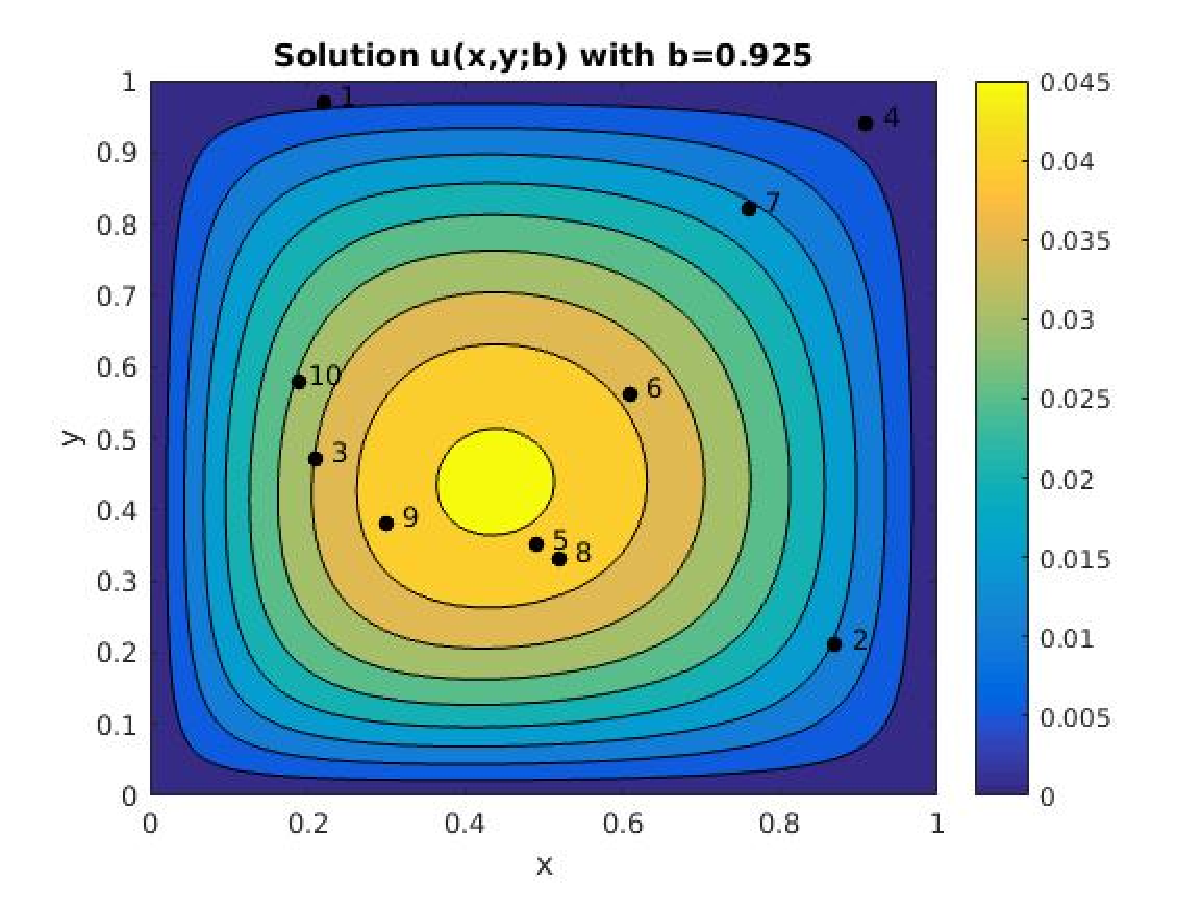
\includegraphics[scale=0.5]{./FigChap3/solu}
\caption{Numerical solution of the system (\ref{eqntoyproblem}) using a finite difference scheme. The mesh
size used in $x$ and $y$ was $0.01$. The value of the parameter $b$ was set at $0.925$. The black dots
in the plot represent the points used to generate the synthetic data about the experimental
measures $m$.}
\label{figsolU}
\end{figure}


At this point  we use the concept of emulator as in the previous chapter. If we had unlimited computational
power or time then we can run the finite difference scheme used to obtain Figure \ref{figsolU} with
a huge set of possible values for $b$ in the interval $(0,2]$. And pick the value that replicates the
better the syntetic data $m$. Since we do not have unlimited computational power or time what we
are going to do is to pick some $n$  values $b_{k}\in (0,2], k=1,2,\ldots,n$, run the finite difference
scheme on those and then use an emulator $\hat{f}$ with GPs to fill the missing data. The criteria to 
choose the number $n$ comes from considerations of how much time and computational resources we have.
For this case we chose $n=10$. How to distribute those 10 points in the interval $(0,2]$. Here we
use the concept space filling design. In the one dimensional setting it is not hard to see that
a maximin design gives an equal spacing of the 10 points in the interval $(0,2]$ hence we choose
\begin{equation*}
b_{k}=0.2k \qquad\text{for }k=1,2,\ldots,10.
\end{equation*}

We are ready to run the emulator $\hat{f}$ for these values of $b$, get a numerical value at
the 10 points in the domain where the synthetic data were created (black dots in Figure \ref{figsolU})
and use GPs to fill the missing information. Take into account that this process of `filling the blanks'
has to be done in all of the 10 measurement points in the domain $\Omega$ of definition of the phyiscal model.

In Figure \ref{fignofitted} we can see the results from running the emulator (black dots) compared
with the experimental measurement for each of the 10 sites (black line).

\begin{figure}[H]
\centering
\includegraphics[scale=0.5]{./FigChap3/nofitted}
\caption{whatever}
\label{fignofitted}
\end{figure}



\bibliography{Tesis}
\bibliographystyle{plain}




\end{document}
